\documentclass[thesis.tex]{subfiles}

\begin{document}

\chapter{Compute Resource Adaptation}
\label{cha:comp-reso-adapt}

In this chapter, we focus on swarm applications with computation-heavy tasks,
such as machine learning (ML) inference. To create an engaging user experience,
these applications need to offer bounded response times (e.g., 100 ms or
sub-second). However, end devices are often not powerful enough to run an
algorithm as is. While applications can offload computation to other resources
such as the edge or the cloud, swarm platforms have a large discrepancy of
computing capabilities. In addition, the edge/cloud faces the challenge of
unpredictable network delays and service overload. To meet the response time
requirement, we propose to adapt computation to each platform.

The ability to adapt comes from the availability of many options to for the same
task: different algorithms or different parameters for the same algorithm. These
options result in different processing times and application accuracy. If we can
build a performance model that characterizes the impact of each option, the
application can choose the right algorithm/parameter adaptively depending on the
available compute power and meet the deadline.

Building this performance model for compute resource adaptation is
challenging. Unlike the profiling discussed in \autoref{cha:netw-reso-adapt},
exhaustive profiling is not viable due to two issues: $(i)$ we are facing
algorithms with more parameters that form a much larger combinatorial space;
$(ii)$ because processing times vary across devices, we need to profile for each
swarm device, even those that are not available at development time but will be
used at deployment.

This chapter is step further in refining our profiling techniques. First, we
address the issue with a large parameter space by employing Bayesian
Optimization (BO). We demonstrate that BO can reduce the number of samples we
need by more than 50$\times$ fewer compared to an exhaustive approach. With the
same search budget, BO finds better Pareto-optimal configurations than random
search and coordinate search. Second, to profile for new devices, we propose to
transfer an existing profile by updating the processing times of Pareto-optimal
configurations. The profile transfer eliminates the need to get all training
data, evaluate the algorithm for all data, and run BO engine.

\section{Introduction}
\label{sec:introduction}

An increasing number of swarm applications rely on heavy computation tasks,
notably machine learning (ML) applications. For example, Microsoft
SeeingAI~\cite{seeingai} is a talking camera for the blind and low vision
community that describes nearby people, text, objects, etc. Wearable cognitive
assistant~\cite{ha2014towards} uses wearable devices, such as Google Glass, for
deep cognitive assistance, e.g., offering hints for social interaction via
real-time scene analysis.

While there is a staggering collection of research focusing on model
\textit{training} for these tasks, for swarm applications, they perform the
\textit{inference} step of machine learning: it uses a trained model to make a
prediction given an input, such as visual~\cite{googlelens, ha2014towards,
  seeingai}, audio~\cite{alexa, applesiri, cortana}, and sensory
information~\cite{laput2017synthetic, lu2010jigsaw}. Inference has received
relatively little attention, especially on edge and end devices.

One important challenge for inference is to bound the response time, which
affects user experience significantly in these human-in-the-loop
systems. Previous usability studies~\cite{nielsen1994usability,
  schneiderman1998designing} have measured the effect of different end-to-end
response times:

\begin{itemize}[noitemsep, topsep=0pt]
\item 100 ms gives the feeling of instantaneous response.
\item 1 second keeps the user's flow of thought but users can sense the delay.
\item A few seconds' delay creates an unpleasant user experience.
\end{itemize}

Achieving bounded response times (BRT) on swarm devices has remained
challenging. Swarm devices are extremely heterogeneous and many are resource
constrained (see \autoref{tab:embedded}). Heavy computations can be simply
beyond the capabilities of cheap end devices. For example, state-of-the-art
object detection algorithm easily takes several seconds on modern
smartphones~\cite{chen2015glimpse}.

To compensate resource-constrained devices, prior work explores
offloading~\cite{chun2011clonecloud,cuervo2010maui} to the cloud or the edge
that hosts machine learning models and performs heavy computation. Despite their
powerful computing capability and more available resources, e.g., special
hardware like GPU and TPU~\cite{jouppi2017datacenter}, these machines suffer
from increased network latency and service overload (\autoref{fig:edge}). As a
result, they are often unable to meet response time goals consistently.

Another technique for low latency is to use redundant requests. By initiating
multiple requests across a diverse set of resources and using the first result
that completes, redundancy is effective to address the variability in network
delays~\cite{gordon2015accelerating, vulimiri2013low} and slow servers (known as
straggler mitigation in the cloud~\cite{dean2013tail,
  ananthanarayanan2013effective}). However, existing works treat these resources
equally and execute the same task on each platform, a poor match for the
heterogeneous swarm space.

We make the observation that for a particular task, there are many options:
different algorithms or tunable parameters for the same algorithm. These options
result in different processing times and application accuracy. If we can adapt
the computation by choosing an option that matches the capability of the device
or satisfy the deadline requirement, we can achieve bounded response times.

The idea of adapting to machines is illustrated in \autoref{fig:dr}. It builds
on top of redundancy but addresses, or rather leverages, the heterogeneity of
swarm devices.  On-device processing can use a simple algorithm if the device is
resource constrained. The device also sends redundant requests to other servers,
e.g., the edge and/or the cloud. Each request contains a service-level objective
(SLO) that describes the deadline and accuracy demand. Upon receiving the
request, the server would admit or reject the request based on the network
delays and its workload. Because of the redundancy, rejection is fine. This is
different from traditional web serving where the server is the single point of
source. At last, the device would use the first response that completes.

\begin{figure}
  \centering
  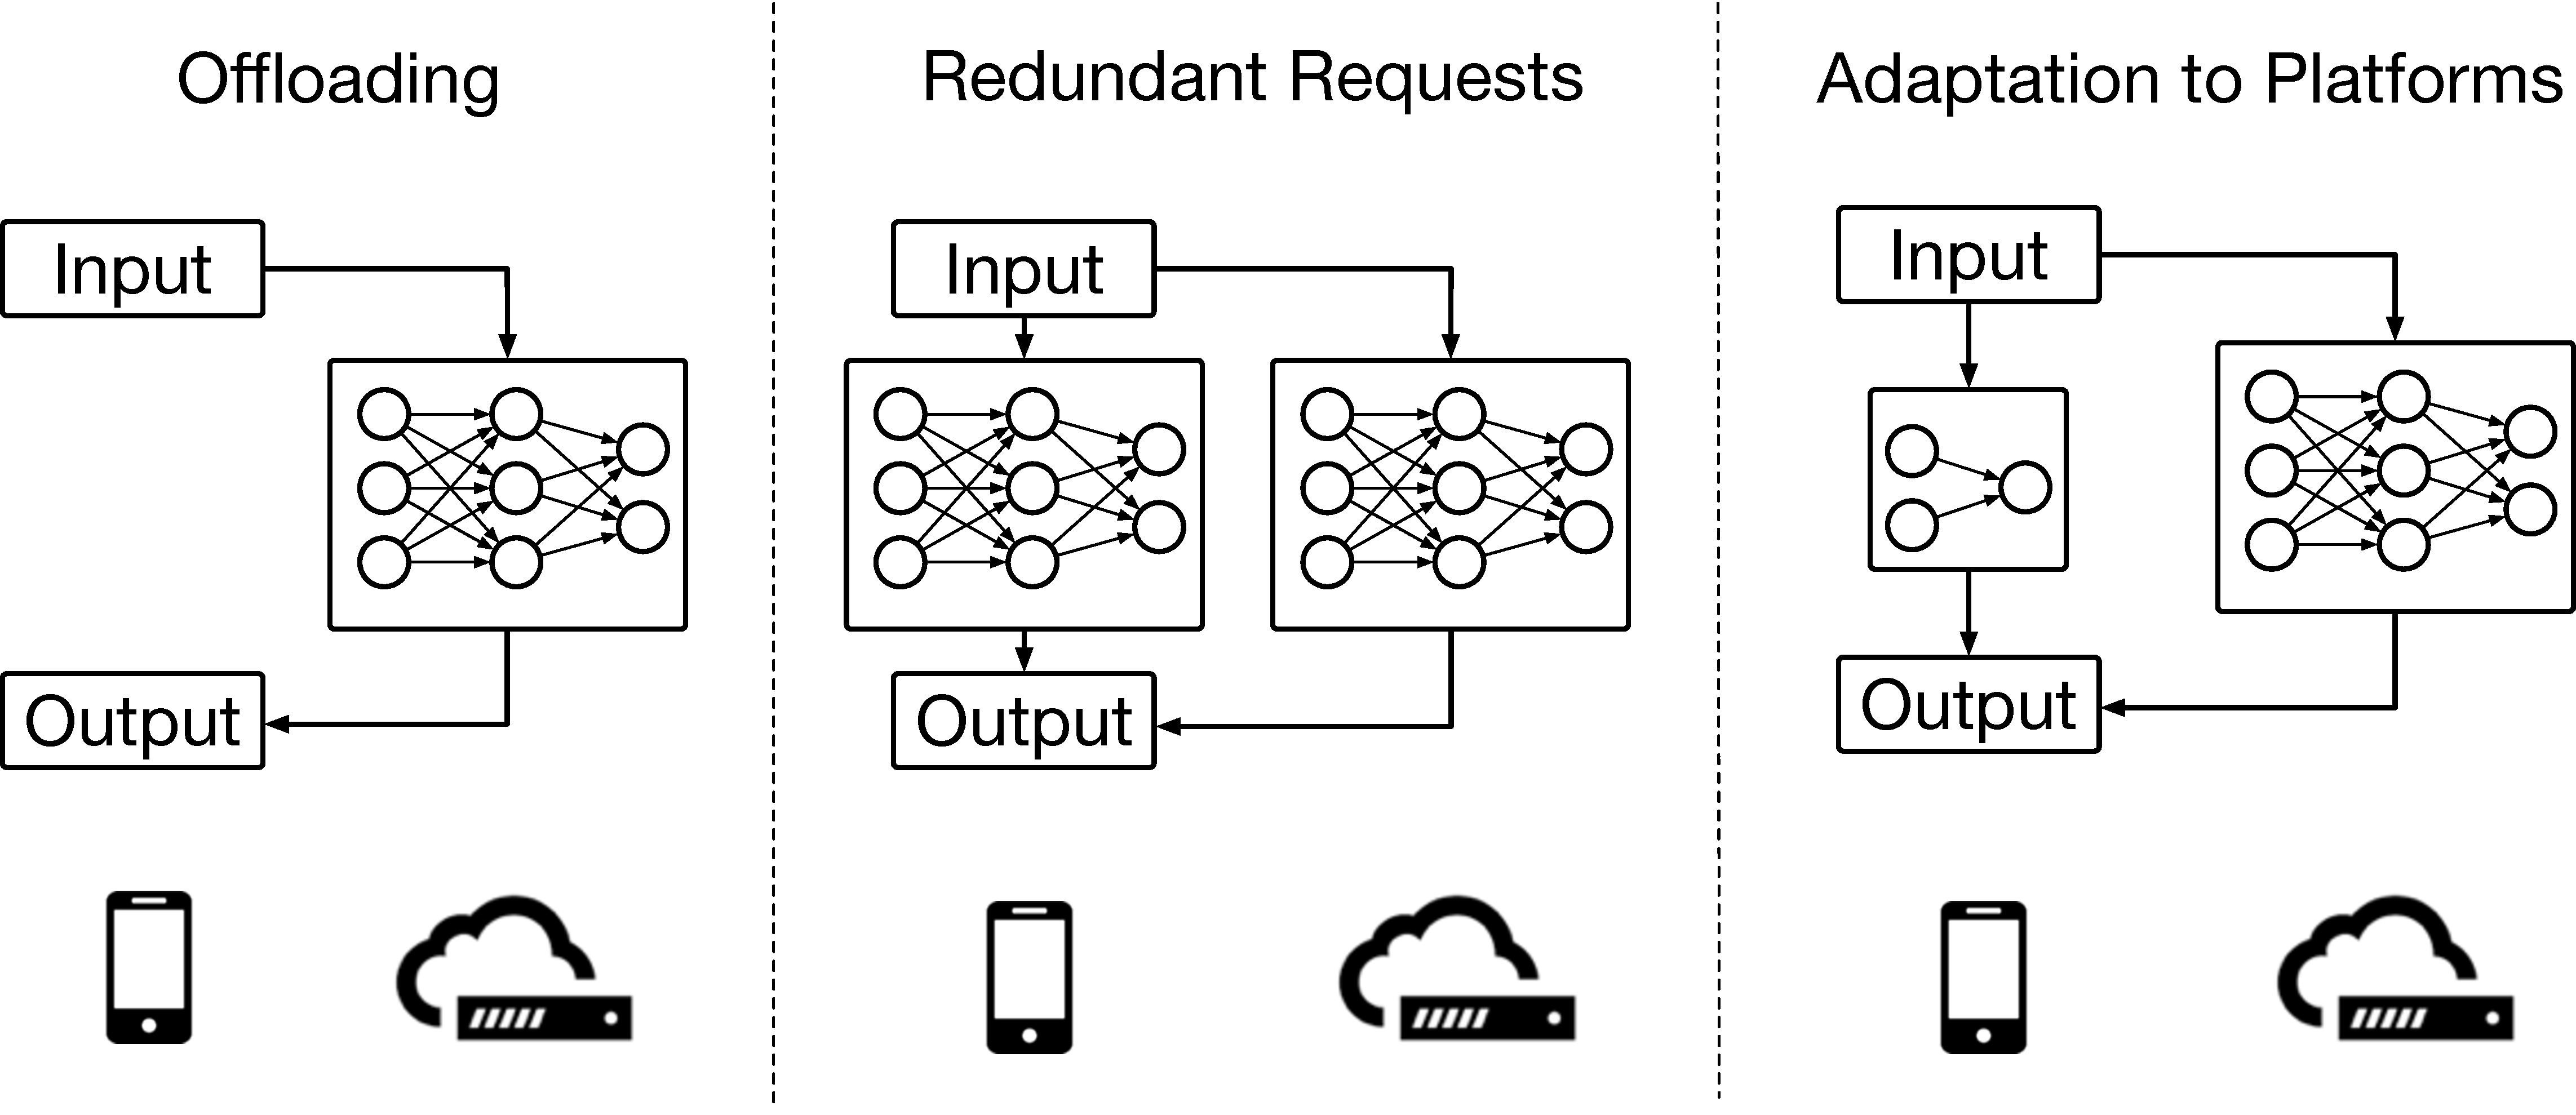
\includegraphics[width=0.8\columnwidth]{figures/dr.pdf}
  \caption{Illustration of offloading, redundant requests and compute
    adaptation.}
  \label{fig:dr}
\end{figure}

The key to enable adaptation lies in building an accurate performance model that
characterized the processing times and accuracy trade-off for a particular
task. We take a data-driven approach by measuring processing times and accuracy
for a given set of training data. We call this process profiling and the
resulting performance model is the profile.

Efficient profiling is challenging given the large space formed by the
combination of algorithms, parameters, and machines. We need to profile each
algorithms individually. For a single algorithm, it may have a huge parameter
space. For example, cascading classifiers in computer vision tasks have
configurable convolution window size, scale factor, and minimum neighbor for non
maximum suppression. Exhaustive profiling this space is prohibitively expensive
(see \autoref{fig:vj-tradeoff}). Because processing times depend on the devices,
the profile is different across devices. It is infeasible to profile all
hardware platforms because of the staggering number of devices and their
availability at development time.

In this chapter, we discuss techniques to efficiently build the performance
model for compute adaptation in an automated, data-driven way. We first describe
our programming language abstractions that allow developers to specify different
algorithms and their parameters. We then build the profiler. \todo{more.}

This chapter make the following contributions regarding performance modeling:

\begin{enumerate}[noitemsep, topsep=0pt]
\item To address the large parameter space, we use Bayesian Optimization (BO)
  for profiling to learn the Pareto-optimal set of parameters. We show that BO
  outperforms baseline approaches, including random search and coordinate
  search.
\item We propose to transfer profiles across devices without running the
  profiling again. New machines only need to sample a fraction of the
  Pareto-optimal set and measure the processing times only.
\end{enumerate}

%%% Local Variables:
%%% mode: latex
%%% TeX-master: "../compute"
%%% End:

\section{Motivations}
\label{sec:motivation}

We focus on computation-heavy ML applications that are beyond the capabilities
of end devices. In this chapter, we will first show the heterogeneity of swarm
platforms for heavy computation and demonstrate that simple offloading does not
provide consistent response times in the presence of network and workload
variation. We then motivate computation adaptation by showing the trade-off
between application accuracy and processing times in two cases: different
algorithms and different parameters. At last, we summarize the challenges
associated with building an accurate performance model.

\subsection{Heterogeneous Environment}

\begin{figure}
  \begin{minipage}{0.4\textwidth}
    \centering
    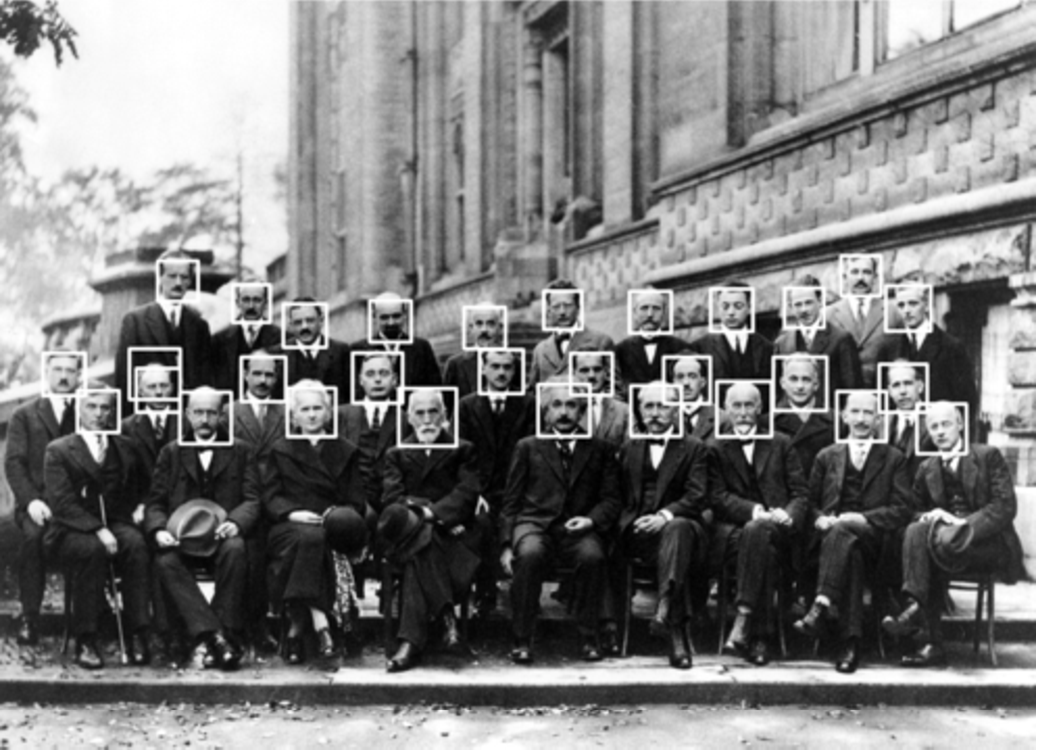
\includegraphics[width=.9\textwidth]{figures/physicist.pdf}
    \label{fig:physicist}
  \end{minipage}%
  \begin{minipage}{0.6\textwidth}
    \centering
    \begin{tabular}{c c c}
      \toprule
      \specialcell{RPi\\Model B}
      & \specialcell{Macbook \\ Model A1502}
      & \specialcell{Workstation\\Xeon E5-1620} \\
      \midrule
      4105 ms & 544 ms & 346 ms \\
      \bottomrule
    \end{tabular}
  \end{minipage}
  \caption{(Left) Face detection with a photograph of the Fifth Solvay
    International Conference on Electrons and Photons. (Right) Processing times
    using Viola-Jones face detector on different machines,with default OpenCV
    parameters.}
  \label{fig:capabilities}
\end{figure}

Our target application environment consists of machines with large range of
computing resources. Earlier, \autoref{sec:swarm-platforms} and
\autoref{tab:embedded} have discussed this dizzying array of machines ranging
from powerful computing units to low-power microcontrollers.  Low-power devices,
such as mobile phones or IoT microcontrollers, are significantly limited in
their processing capabilities. Performing ML inference easily takes seconds to
complete. As shown in \autoref{fig:capabilities}, to detect faces in a photo of
the Fifth Solvay International Conference on Electrons and Photons,\footnote{The
  original image (3000$\times$2171 pixels) is from Wikimedia and in the public
  domain.} it takes more than 4 seconds on a Raspberry Pi (Model B).

One technique is to use the edge and/or the cloud for offloading. While they are
substantially more powerful (7.5$\times$ to 11.9$\times$ in the face detection
task), both the edge and the cloud suffer from variable latency, unstable
connection, and service contention. These issues make it difficult to provide
consistent response times, especially for tail performance. \autoref{fig:edge}
shows the characteristics of end devices, the edge, and the cloud. We then
empirically validate the network variation and workload variation
(\autoref{fig:variation}).

\para{Network Variation.} We use the raw data in January 2016 from FCC
\href{https://www.fcc.gov/general/measuring-broadband-america}{Measuring
  Broadband America Program}~\cite{fcc} to validate the large variation in wide
area network. \autoref{fig:fcc-latency} shows the empirical cumulative
distribution function (ECDF) of measured network latency. \textit{Ping} time refers to
the round trip time (RTT) of ICMP echo requests from measurement devices to a
set of target test nodes. \textit{Download} and \textit{Upload} are latency
measured when performing downstream or upstream speed tests. From this figure,
we can see that the latency has 2-3 orders of magnitude difference. The
situation is worse with active traffic. The median network delay increases from
\SI{22}{\ms} to \SI{80}{\ms} under downstream load and \SI{272}{\ms} under
upstream load.

\para{Workload Variation.} \noindent We measure end-to-end latency with
TensorFlow serving~\cite{olston2017tensorflow}, a state-of-the-art serving
system for machine learning models. Specifically, we use
MNIST~\cite{lecun1998mnist} as a case study and study the serving performance
with different level of background load. \autoref{fig:tf-latency} shows the ECDF
with no load, 1K requests per second (RPS) and 5K RPS. From this figure, we can
see that the serving latency has significantly increased when the load
increases. With 1k load, 99.9 percentile latency increases from \SI{3.5}{\ms} to
\SI{22.5}{\ms}. With 5K load, even the median latency increases to
\SI{21.5}{\ms}: a 22.4$\times$ increase from \SI{0.96}{\ms} with no load.

\begin{figure}
  \centering
  \begin{subfigure}[t]{0.4\columnwidth}
    \centering
    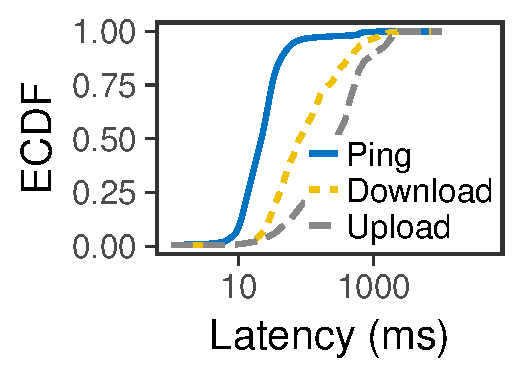
\includegraphics[width=\textwidth]{figures/fcc_latency.pdf}
    \caption{Broadband network latency.}
    \label{fig:fcc-latency}
  \end{subfigure}
  \hspace{2em}
  \begin{subfigure}[t]{0.4\columnwidth}
    \centering
    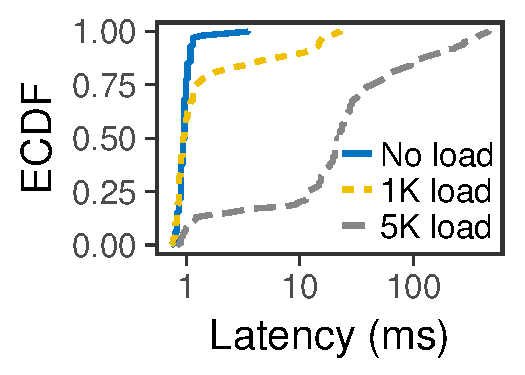
\includegraphics[width=\textwidth]{figures/tf_latency.pdf}
    \caption{TensorFlow serving latency.}
    \label{fig:tf-latency}
  \end{subfigure}
  \caption{(Left) WAN network latency has variation and the latency deteriorates
    during downstream and upstream speed tests. (Right) Server processing
    latency has variation and the latency deteriorates during load increase.}
  \label{fig:variation}
\end{figure}

\subsection{Accuracy-Time Trade-off}
\label{sec:comp-perf-model}

\begin{figure}[t]
  \centering
  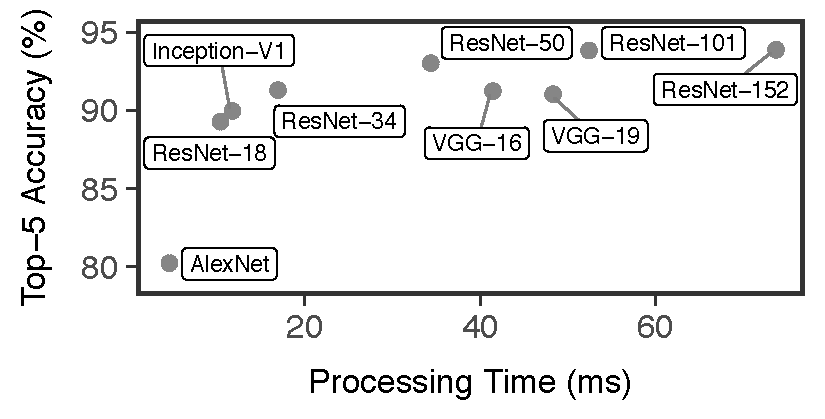
\includegraphics[width=.7\columnwidth]{figures/tradeoff-cnn.pdf}
  \caption{Benchmarks for popular CNN models demonstrate the trade-off between
    application accuracy and processing times. For data source and details,
    refer to
    \href{https://github.com/jcjohnson/cnn-benchmarks}{cnn-benchmarks}~\cite{cnn.benchmarks}.
  }
  \label{fig:cnn-tradeoff}
\end{figure}

Many tasks, especially ML inference, have multiple algorithms, or tunable
parameters for the same algorithm. These options result in different application
accuracy and processing times. As a result, we can speed up a computation task
by sacrificing accuracy. In this way, many tasks become tractable on end
devices. Servers can also tune their computation to accommodate network delays
or address heavy load. Below we show two examples.

\para{Convolutional Neural Networks (CNN)}. For the past few years, deep
learning and neural networks have gained attention in performing complex machine
learning tasks~\cite{goodfellow2016deep}. Convolutional neural networks (CNNs)
are particularly powerful for computer vision tasks, such as object detection
and image classification. There are many networks available:
AlexNet~\cite{krizhevsky2012imagenet}, Inception~\cite{szegedy2015going},
VGG~\cite{simonyan2014very}, ResNet~\cite{he2016deep}, etc. Huang et al. have
observed the speed/accuracy trade-off and explored this trade-off in an
exhaustive and fair manner~\cite{huang2016speed}. Because this thesis is not an
extensive study of neural networks, we only summarize one benchmark result in
\autoref{fig:cnn-tradeoff}. The processing times vary from \SI{4.3}{\ms} to
\SI{73.5}{\ms} and the accuracy\footnote{Top-5 accuracy here means that the
  correct label is one of the top five predictions made by the network.} varies
from 80.2\% to 93.8\%.

\para{Viola-Jones Face Detector.} This is an example of how tunable parameters
affect processing times and application accuracy. Viola-Jones (VJ) face
detector~\cite{viola2001rapid} detects face by moving a window over the image.
To detect faces at different sizes, it runs over an image pyramid with a
configurable scale. After the detection, there are typically multiple
neighboring windows with high scores close to the correct location of objects.
A post-processing step uses non-maximum suppression (NMS) to group detection
into a single bounding box. OpenCV~\cite{opencvlibrary} provides
\texttt{CascadeClassifier} with the following parameters,

\begin{itemize}[noitemsep, topsep=0pt]
\item \texttt{min\_size}: minimum detectable object size.
\item \texttt{scale}: how much image size is reduced at each image scale.
\item \texttt{min\_neighbors}: how many neighbors each candidate rectangle should
  have to retain it.
\end{itemize}

\begin{figure}[t]
  \centering
  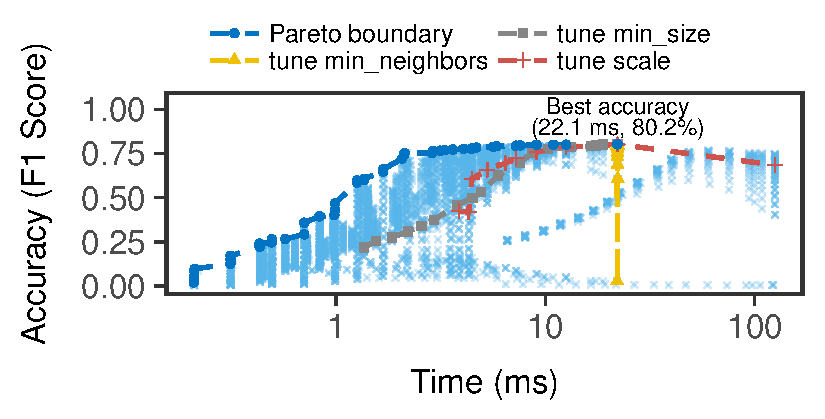
\includegraphics[width=.8\columnwidth]{figures/exhaustive-face.pdf}
  \caption{Benchmarks for Viola-Jones face detector with different
    parameters. These parameters form a large space that make performance
    modeling challenging.}
  \label{fig:vj-tradeoff}
\end{figure}

\autoref{fig:vj-tradeoff} shows how these parameters affect processing times and
accuracy. We measured the performance of 4,000 different parameter
configurations\footnote{\texttt{min\_size} ranges from 0 to 190, with a step
  size of 10; \texttt{scale} ranges from 1.01 to 1.46, with a step size of 0.05;
  \texttt{min\_neighbors} ranges from 0 to 19, with a step size of 1.} using
FDDB dataset~\cite{jain2010fddb}. In the figure, each cross dot represents the
processing time and application accuracy for one configuration. As we can see,
there is a trade-off space: the processing times vary across almost 3 orders of
magnitude; the accuracy can be as low as 0\% and as high as 80.2\%.

% scale factor: 1.01..0.05..1.46 (10)
% min neighbors: 0..1..19
% min size: 0..10..190

\subsection{Performance Modeling and Challenges}
\label{sec:perf-model-chall}

We need to build the performance model to exploit the trade-off between accuracy
and processing times. Because each algorithm is fundamentally different from
another one, we must exhaustively evaluate all available algorithms. For the
same algorithm with different parameters, exhaustive search can be prohibitively
expensive as the parameters form a combinatorial
space. \autoref{fig:vj-tradeoff} shows an evaluation of 4,000 parameter
configurations for Viola-Jones, which only has three parameters. A more complex
algorithm can have a staggering number of tunable parameters. For example,
HOG~\cite{dalal2005histograms} in OpenCV has the following parameters:
\texttt{win\_size}, \texttt{win\_stride}, \texttt{block\_size},
\texttt{block\_stride}, \texttt{cell\_size}, \texttt{nbins},
\texttt{win\_sigma}, \texttt{nlevels}, \texttt{hit\_threshold},
\texttt{padding}, \texttt{group\_threshold}, \texttt{use\_meanshift\_grouping},
etc.

A comprehensive performance modeling is actually not necessary. Instead, we only
need configurations that provide the best accuracy for a given processing time
constrain, i.e., the Pareto-optimal points. \autoref{fig:vj-tradeoff} highlights
the Pareto boundary in blue. We defer a formal definition of the Pareto-optimal
set in \autoref{sec:profiling-formalism}.

In practice, we can reduce the number of samples further. The Pareto-optimal set
only needs to be accurate enough to distinguish near-optimal configurations from
the rest. Previous work has used two solutions: $(i)$ \textit{Random search.}
This simple approach samples the parameter space randomly and search/profile
with a budget. It is obvious that as the budget increases, the coverage improves
and the Pareto-optimal set is closer to the correct set. $(ii)$
\textit{Coordinate search.} This greedy approach starts with a random
configuration, moves along one parameter dimension if it improves, and stops
when it reaches a local optimum. After reaching the local optimum, if we still
have search budget, this approach repeats by picking another random
configuration.

Both random search and coordinate search have their problems. Random search
needs a lot of samples to approximate the real Pareto boundary. Coordinate
search may stuck in some local region and exhaust the search budget. As a
result, with a limit budget, both approaches could return sub-optimal points in
the trade-off space.

In addition, our discussion on performance modeling by far has not taken into
account of the heterogeneous capabilities of devices. What we have shown in
\autoref{fig:vj-tradeoff} is measured on a workstation with Xeon E5-1620 CPU;
the performance model will be different on another device, e.g., a Raspberry Pi.

%%% Local Variables:
%%% mode: latex
%%% TeX-master: "../compute"
%%% End:

\section{Learning the Pareto-optimal Set Efficiently }
\label{sec:learn-pareto-optim}

In this section, we discuss techniques that learns the Pareto-optimal set
efficiently. We first describe our programming abstraction and profiling
formalism. We then focus on addressing two profiling challenges: the large
parameter space and device heterogeneity. $(i)$ We propose to use Bayesian
Optimization (BO) to address large parameter space with multiple parameters. And
we show that it outperforms previous approaches (random search and coordinate
search). $(ii)$ We propose to use profile transfer to derive the profile for a
new device without running expensive profiling from scratch.

\subsection{Programming Abstraction for Compute Adaptation}
\label{sec:progr-abstr}

Unlike \autoref{sec:structure-adapt}, the algorithms and parameters do not come
from a series of chained operators. Therefore, we need new programming
abstractions. However, the design goal is similar: to free developers from
specifying exact rules and allow specifications with options.

We use \texttt{trait}\footnote{\texttt{trait} in Rust is similar to
  \texttt{interface} in other languages.} to abstract each algorithm, as below:

\begin{lstlisting}[xleftmargin=.1\textwidth, xrightmargin=.1\textwidth, language=Rust]
trait Algorithm {
    type I;
    type O;
    type P;
    fn execute(&mut self, i: &Self::I, p: &Self::P) -> Self::O;
}
\end{lstlisting}

Each algorithm is specified by its input data type \texttt{I}, output data type
\texttt{O}, a parameter type \texttt{P}, and its behavior function
\texttt{execute}. For any data type \texttt{T} that implements
\texttt{Algorithm} trait, the function \texttt{execute} can access the internal
data structure of \texttt{T} in a mutable way: \texttt{\&mut self}. Type
\texttt{I}, \texttt{O}, and \texttt{P} are abstract types and the implementation
must specify the concrete types. We show an implementation of Viola-Jones in
\autoref{fig:vj} where the input type is an image, the output type is a
detection, and the parameter is \texttt{VJParameters}. When composing
algorithms, their input data type and output data type must match. This type
constrain is used to validate that two algorithms are performing the same
task. Their parameters can be different.

For tunable parameters, we need to be able to specify at least three parts:
\texttt{min}, \texttt{max}, and \texttt{step}. We extend an algorithm's
parameter by augmenting it with macros annotations. In Rust, this can be
implemented with procedural macros as a syntax extension. \autoref{fig:vj} shows
these annotation in blue: we use \texttt{\#[derive(Adapt)]} to mark that this
\texttt{struct} is a tunable parameter and use \texttt{\#[adapt(...)]} to mark
its field.

\begin{figure}
  \centering
\begin{lstlisting}[language=Rust]
#[derive(Adapt)]
struct VJParameters {
    #[adapt(min = "0", max = "20", step = "1")]
    min_neighbors: i64,

    #[adapt(min = "0", max = "190", step = "10")]
    min_size: i64,

    #[adapt(min = "1.01", max = "1.5", step = "0.01")]
    scale_factor: f64,
}

struct VJ {
  // ... omitted ...
}

impl Algorithm for VJ {
    type I = Image;
    type O = Detection;
    type P = VJParameters;

    fn execute(&mut self, image: &Image, opt: &VJParameters) -> Detection {
        // ... omitted ...
    }
}
\end{lstlisting}
  \caption{Viola-Jones face detector parameters \texttt{VJParameters} annotated
    with adaptation. \texttt{VJ} implements the \texttt{Algorithm} trait.}
  \label{fig:vj}
\end{figure}

\subsection{Profiling Formalism}
\label{sec:profiling-formalism}

The goal of profiling is to build a profile that characterizes the trade-off
between application accuracy and processing times such that for a running
application, it can choose the right algorithm/parameter to meet the
deadline. As discussed in \autoref{sec:perf-model-chall}, we are only interested
in the Pareto-optimal set.

We start with defining the Pareto-optimal set for a specific algorithm with
varying parameters. For an algorithm with $n$ parameters, e.g., $n$ is 3 for
Viola-Jones, we call each parameter a knob and refer it as $k_i$. The
combination of all knobs forms a parameter \textit{configuration}
$c = [k_{1}, k_{2}, ... k_{n}]$. The set of all possible configurations
$\mathbb{C}$ is the space that the profiling explores for this algorithm. For
each configuration $c$, we are interested in two mappings: a mapping from $c$ to
its processing times $T(c)$ and its accuracy measure $A(c)$.  The profiling
looks for Pareto-optimal configurations; that is, for any configuration $c$ in
the Pareto-optimal set $\mathbb{P}$, there is no alternative configuration $c'$
that requires a smaller processing time and offers a higher accuracy. Formally,
$\mathbb{P}$ is defined as follows:

{\small \vspace{-1em}
  \begin{equation}
    \mathbb{P} = \{ c \in \mathbb{C} : \{ c' \in \mathbb{C}: T(c') < T(c),
    A(c') > A(c) \} = \varnothing\}
  \label{eq:pareto2}
\end{equation}
}%

Once we have the Pareto-optimal set for one algorithm, we can compose multiple
algorithms and merge their Pareto-optimal set by finding the global
Pareto-optimal configurations. Both processing times and application accuracy
are simply real numbers and can be compared, although each algorithm's parameter
may be completely different.

\subsection{Profiling Parameters with Bayesian Optimization}
\label{sec:prof-param-with}

Bayesian Optimization (BO)~\cite{snoek2012practical} is a technique that
approximates black-box functions with proxy functions, iteratively proposes new
sample point to evaluate in the large parameter space, and finds the global
maximum (or minimum). It is effective for black-box functions when evaluating
each sample is expensive and noisy, such as tuning parameters and model
hyperparameters in ML tasks~\cite{snoek2012practical}. A comprehensive review of
BO is beyond the scope of this thesis. We briefly describe what BO brings using
an example without going into the gory details.

\begin{figure}
  \begin{subfigure}{\textwidth}
    \centering
    
\includegraphics[width=0.5\textwidth]{figures/bo-legend.pdf}
  \end{subfigure}
  \vspace{0.2em}
  \\
  \centering
  \begin{subfigure}{0.45\textwidth}
    \centering
    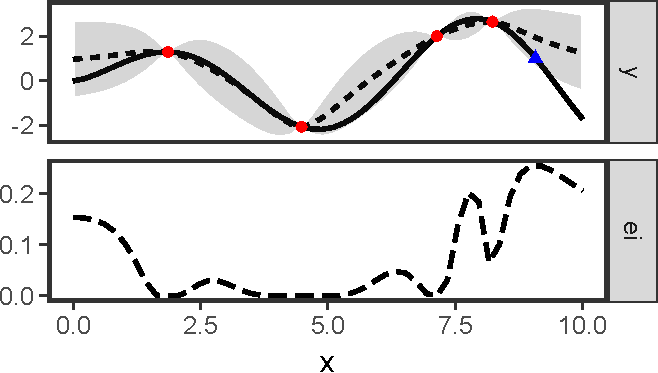
\includegraphics[width=\textwidth]{figures/bo1.pdf}
    \caption{First Iteration.}
  \end{subfigure}
  \hspace{1em}
  \begin{subfigure}{0.45\textwidth}
    \centering
    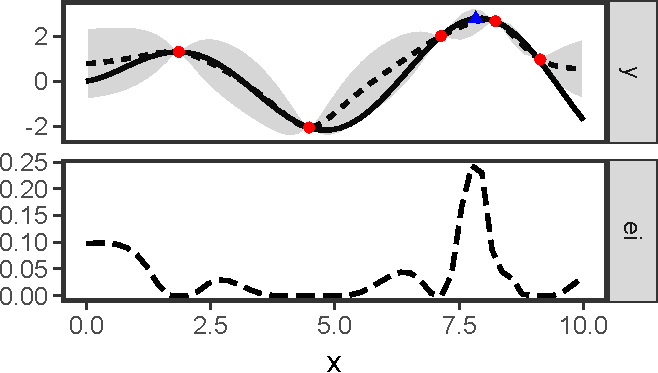
\includegraphics[width=\textwidth]{figures/bo2.pdf}
    \caption{Second Iteration.}
  \end{subfigure}
  \caption{Bayesian Optimization illustrated.}
  \label{fig:bo-1d}
\end{figure}

\autoref{fig:bo-1d}, produced with the mlrMBO package~\cite{bischl2017mlrmbo},
illustrates the process of finding the maximum point for 1-dimension Alpine N. 2
function~\cite{clerc1999swarm}. The solid line labeled $y$ is the target
black-box function. The red dots represent samples that have been evaluated. BO
reconstructs a function that best fits these observed samples: the dashed line
$\hat{y}$ (yhat) along with the confidence region (in grey shade).  BO then uses
an acquisition criteria to determine how to sample the next point.  In this
example, it uses expected improvement (EI, in long-dashed line) that balances
high objective (exploitation) and high uncertainty
(exploration)~\cite{shahriari2016taking}. The next proposed sample is the point
that maximizes EI (blue triangles). Running this process iteratively, BO is able
to solve the maximization problem of a black-box function.

% (2.808119, 7.92)

BO recently has been used beyond ML scope.
CherryPick~\cite{alipourfard2017cherrypick} uses BO to find the near-optimal
cloud configurations for big data analytics, i.e., minimizing the cost of
execution. Google uses BO to optimize chocolate chip cookies
recipes~\cite{solnik2017bayesian}, i.e., maximizes the tastiness.

Our problem is more complex as we are solving multi-objective optimizations
(MOO). Specifically, it has two objectives: application accuracy and processing
times. It is trivial to maximize application accuracy or minimize processing
times alone. Previous approaches often transform multiple objectives into a
single objective using scalarization techniques: using weighted sum to combine
different objectives. These approaches are expected to be
sub-optimal~\cite{knowles2006parego}. Recent research progress has made the
transformation unnecessary. We can directly consider the Pareto-optimal set and
evaluate the improvements with different acquisition criteria: $(i)$ additive
epsilon~\cite{binoisgpareto}, $(ii)$ hypervolume~\cite{binoisgpareto}; $(iii)$
the entropy of the posterior distribution over the Pareto-optimal
set~\cite{hernandez2016predictive}. We illustrate the first two criteria in
\autoref{fig:bo-2d}. We use PESMO~\cite{hernandez2016predictive} because of its
availability and ease of use. It is available within the Spearmint
package~\cite{snoek2016spearmint}.  PESMO also has a low computational cost: it
grows linearly with respective to the total number of objectives $K$.

\begin{figure}
  \centering
  \begin{subfigure}{0.45\textwidth}
    \begin{tikzpicture}
      \pgfplotstableread{
        0 0.1 -0.1
        0 0.1  0.2
        1 0.25 0.5
        2 0.4  0.6
        3 0.5  0.85
        4 0.9  0.9
        4 1.2  0.9
      }\datatable
      \begin{axis}[
        width  = \textwidth,
        xlabel = Processing Times (normalized),
        ylabel = Accuracy,
        axis line style = thick,
        ymin   = 0,
        ymax   = 1,
        ytick  = {0, 0.2, 0.4, 0.6, 0.8, 1},
        xmin   = 0,
        xmax   = 1,
        xtick  = {0, 0.2, 0.4, 0.6, 0.8, 1},
        ]

        \addplot+[red!50,
        mark size=3pt, mark options={draw=red!0, fill=red!80}, const
        plot mark left, thick] table [x index=1, y index=2]{\datatable};

        \addplot[mark=triangle*, mark options={draw=blue!80, fill=blue!80},
        mark size=3pt, fill=blue!80, only marks]
        coordinates { (0.3, 0.7) };

        \draw[-, blue, dashed] (axis cs:0.3, 0.5) -- (axis cs:0.3, 0.7);
        \draw[-, blue, dashed] (axis cs:0.3, 0.7) -- (axis cs:0.5, 0.7);
        \draw[<->, >=stealth, blue] (axis cs:0.45, 0.6) -- (axis cs:0.45, 0.7);
        \draw[<->, >=stealth, blue] (axis cs:0.3, 0.55) -- (axis cs:0.4, 0.55);

      \end{axis}
    \end{tikzpicture}
  \end{subfigure}
  \hspace{1em}
  \begin{subfigure}{0.45\textwidth}
    \begin{tikzpicture}[
      triangle/.style = {fill=blue!80, regular polygon, regular polygon sides=3}
      ]

      \pgfplotstableread{
        0 0.1 -0.1
        0 0.1  0.2
        1 0.25 0.5
        2 0.4  0.6
        3 0.5  0.85
        4 0.9  0.9
        4 1.2  0.9
      }\datatable
      \begin{axis}[
        width  = \textwidth,
        xlabel = Processing Times (normalized),
        ylabel = Accuracy,
        axis line style = thick,
        ymin   = 0,
        ymax   = 1,
        ytick  = {0, 0.2, 0.4, 0.6, 0.8, 1},
        xmin   = 0,
        xmax   = 1,
        xtick  = {0, 0.2, 0.4, 0.6, 0.8, 1},
        axis on top
        ]

        \addplot+[blue!50, no marks,
        mark size=3pt, mark options={draw=blue!0, fill=blue!80},
        % pattern=north east lines,
        % pattern color=blue!50,
        fill=blue!20,
        ]
        coordinates {(0.3, 0.5) (0.3, 0.7) (0.5, 0.7) (0.5, 0.6) (0.4, 0.6)
          (0.4, 0.5) (0.3, 0.5)};

        \addplot+[red!50, mark=*,
        mark size=3pt, mark options={draw=red!0, fill=red!80}, const
        plot mark left, thick,
        pattern=north west lines,
        pattern color=red!50]
        table [x index=1, y
        index=2]{\datatable} \closedcycle;

        \addplot[mark=triangle*, mark options={draw=blue!80, fill=blue!80},
        mark size=3pt, fill=blue!80, only marks]
        coordinates { (0.3, 0.7) };

      \end{axis}
    \end{tikzpicture}
  \end{subfigure}
  \caption{To find the Pareto-optimal set that maximizes accuracy while
    minimizing processing times, the acquisition criterion can suggest new
    samples (blue triangles) to the current Pareto-optimal set (red points) by
    maximizing additive epsilon (left, blue arrows) or hypervolume (right, blue
    shade area). This illustration is adapted from GPareto
    vignette~\cite{binoisgpareto}.}
  \label{fig:bo-2d}
\end{figure}

%%% Local Variables:
%%% mode: latex
%%% TeX-master: "../compute"
%%% End:


We then show that BO can effectively explore the large design space and come up
with a better Pareto-optimal set. We compare BO with two baseline approaches:
$(i)$ random search; $(ii)$ coordinate search.

For coordinate search, because it is a greedy approach, the original two
objectives is converted into one single objective: $X(c) = A(c) - \beta
T(c)$. We augment the basic version of the coordinate search with a few
techniques: $(i)$ to avoid starting with an expensive configuration and
exploring its neighbors, we pick $m$ random configurations and start from the
one with the highest $X$. VideoStorm~\cite{zhang2017live} suggests that even
$m = 3$ can successfully avoid starting in an expensive part of the search
space. $(ii)$ because $\beta$ affects the relative impact of $T$ and $A$, we
change its value once we have found a global maximum and still have search
budget.

\autoref{fig:bo} shows the evaluation results using Viola-Jones face detector
and FDDB dataset. With similar search budgets, the Pareto-optimal set BO finds
is better than the baseline approaches. We can see that coordinate search is
relatively dense in some area as it moves slowly from one point to its
neighbors. Random search has a better coverage of the space, but to find a
better Pareto front, it needs more samples.

\begin{figure}
  \centering
  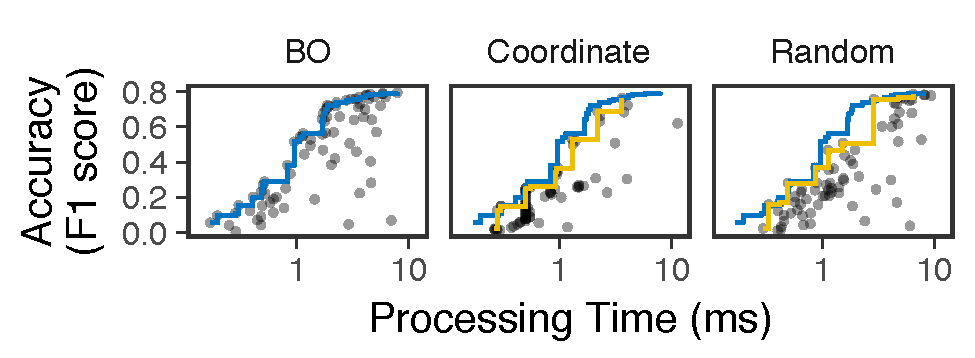
\includegraphics[width=0.85\columnwidth]{figures/bo-eval.pdf}
  \caption{Using Viola-Jones as an example, BO evaluates 50 configurations and
    recommends 29 configurations as the Pareto-optimal boundary (the blue line
    in all subfigures). Greedy and Random find sub-optimal Pareto configurations
    with a budget of 80 evaluations (the yellow line in each figure).}
  \label{fig:bo}
\end{figure}

\subsection{Profile Transfer Across Devices}
\label{sec:performance-transfer}

The profile we learned is specific to the devices. While it seems that we need
to profile for every device, the profiling problem can be simplified. The
insight lies in the properties of our objectives. $A(c)$ doesn't change across
devices. We assume $T(c)$ is monotonic across devices, that is, a slower devices
remains slower for different configurations. Mathematically, if $T_1$ and $T_2$
are the mappings from configurations to processing times on two devices, the
monotonic property means that if $T_1(c') < T_1(c)$, then $T_2(c') < T_2(c)$.

As a result, it is easy to see that the same configuration $c$ remains in the
Pareto-optimal set $\mathbb{P}$ regardless of what devices the algorithm runs
on. So the whole Pareto-optimal set can be transferred. Visually, the profile on
the second device is a stretched or shrunk version from a reference device along
the dimension of processing times.

This simplifies our performance modeling on a new device. We only need to
measure processing times of the Pareto-optimal set. And measuring processing
times is significantly easier than measuring accuracy. One do not need to gather
all the training data, run the algorithm, compare it with the ground-truth, and
calculate the accuracy. The transfer can be further simplified if we use a
linear transformation to approximate the relationship between processing times
on two platforms. In this way, we only need to measure processing times from two
configurations.

We empirically validate profile transfer on three devices with Viola-Jones face
detector (\autoref{fig:transfer}). We use the profile learned on a reference
machine and evaluate the processing times on two target machines. The left
figure shows that a near-linear relationship between the process times on two
machines. The right figure shows the stretched/shrunk effect of the profile. In
this figure, we use the average processing times by running all the data. In
practice, a new machine only needs to evaluate a few samples.

\begin{figure}
  \centering
  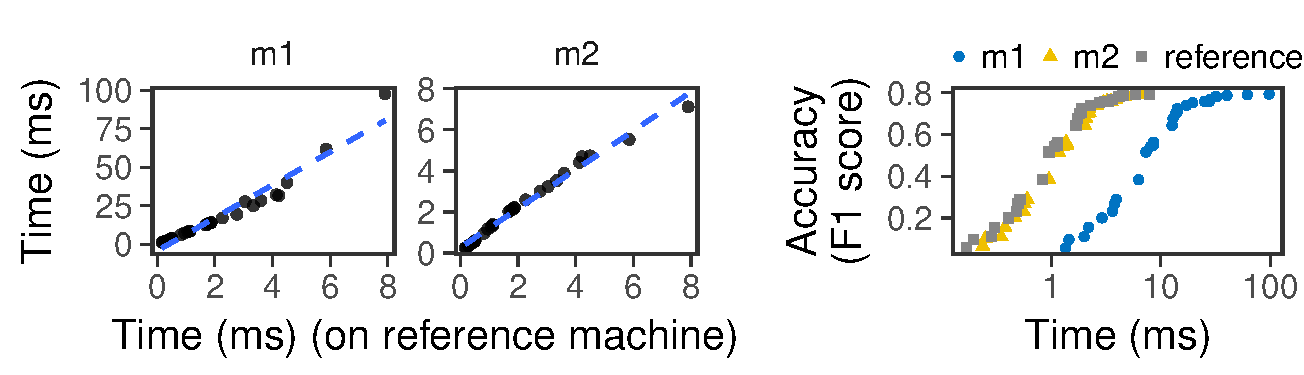
\includegraphics[width=0.9\linewidth]{figures/serving-cross-platform.pdf}
  \caption{(Left) Empirically, processing times follows a linear
    approximation. (Right) Stretched/compressed profile. See paper for
    details.}
  \label{fig:transfer}
\end{figure}

%%% Local Variables:
%%% mode: latex
%%% TeX-master: "../compute"
%%% End:

\section{Discussion}
\label{sec:brt-discussion}

\para{More case studies.} This chapter demonstrates the effectiveness of BO
(\autoref{fig:bo}) and profile transfer (\autoref{fig:transfer}). Our evaluation
uses Viola-Jones face detector, a popular computer vision algorithm, as the
primary case study. We have also applied our profiling to
HOG~\cite{dalal2005histograms} and the results are similar (hence omitted from
this thesis). In the future, we expect to conduct more case studies with diverse
algorithms.

\para{Server scheduling.} Our current use of the profile is simple: we find the
algorithm/parameter that maximizes application accuracy given a processing time
deadline. We envision that in a model serving system that handles a large number
of requests, the profile can help with scheduling, e.g., the server tune
processing times for some requests in order to maximize throughput.

%%% Local Variables:
%%% mode: latex
%%% TeX-master: "../compute"
%%% End:

\section{Chapter Summary}
\label{sec:chap-summary}

We have presented our study of enabling adaptation toward compute resources in
the swarm space. Because end devices are limited in compute power, the
edge/cloud suffer from variable network delays and service requests, it is
essential to be able to adapt computation on different platform to meet response
time deadlines.

To allow the adaptation, we need a performance model that characterizes the
trade-off between application accuracy and processing times. Performance is
challenging: for the large parameter space, previous approaches use random
search or coordinate/greedy approach. and we propose Bayesian Optimization (BO)
for profiling; (2) for heterogeneous computing capabilities and not available
when profiling, we use profile transfer: refine existing Pareto-optimal points.

%%% Local Variables:
%%% mode: latex
%%% TeX-master: "../compute"
%%% End:


\end{document}

%%% Local Variables:
%%% mode: latex
%%% TeX-master: t
%%% End:
